\section{Anhang}
\label{sec:Anhang}

\begin{table}[htbp]
	\centering
	\caption{Messdaten zur langen Spule mit $l = \SI{8,5}{\cm}$.}
	\label{tab:KurzeSpule}
	\begin{tabular}{c c}
		\toprule
		$x / \si{m} $ & $ B / 10^{-3} \si{\tesla}$ \\
		\midrule
		-0,19 & 0,150 \\
		-0,18 & 0,225 \\
		-0,17 & 0,363 \\
		-0,16 & 0,604 \\
		-0,15 & 1,168 \\
		-0,14 & 1,784 \\
		-0,13 & 2,122 \\
		-0,12 & 2,174 \\
		-0,11 & 2,048 \\
		-0,10 & 1,622 \\
		-0,09 & 0,957 \\
		-0,08 & 0,565 \\
		-0,07 & 0,298 \\
		-0,06 & 0,195 \\
		-0,05 & 0,138 \\
		-0,04 & 0,112 \\
		-0,03 & 0,096 \\
		\bottomrule
	\end{tabular}
\end{table}

\begin{table}[htbp]
	\centering
	\caption{Messdaten zur ersten Abstand mit $d_{1} = \SI{7}{\cm}$.}
	\label{tab:ErsterAbstand}
	\begin{tabular}{c c}
		\toprule
		$x / \si{cm} $ & $ B / \si{\milli\tesla}$ \\
		\midrule
	     0,8 &	2,027 \\
	     0,9 &	2,027 \\
	     1,0 &  2,027 \\
	     1,1 &	2,027 \\
	     1,2 &	2,028 \\
	     1,3 &	2,027 \\
	     1,4 &	2,027 \\
	     1,5 &	2,028 \\
	     1,6 &	2,027 \\
	     1,7 &	2,028 \\
	     1,8 &	2,028 \\
	     1,9 &	2,028 \\
	     2,0 &  2,027 \\
	     2,1 &	2,028 \\
	     2,2 &	2,027 \\
	     2,3 &	2,027 \\
	     2,4 &	2,027 \\
	     2,5 &	2,026 \\
	     \midrule
	     7,8  &	1,379 \\
	     8,0  & 1,326 \\
	     8,2  &	1,286 \\
	     8,4  &	1,240 \\
	     8,6  &	1,198 \\
	     8,8  &	1,168 \\
	     9,0  & 1,121 \\
	     9,2  &	1,091 \\
	     9,4  &	1,037 \\
	     9,6  &	1,006 \\
	     9,8  &	0,965 \\
	     10,0 & 0,925 \\
	     10,2 &	0,885 \\
	     10,4 &	0,854 \\
	     10,6 &	0,823 \\
	     10,8 &	0,786 \\
	     11,0 & 0,757 \\
		\bottomrule
	\end{tabular}
\end{table}

\begin{table}[htbp]
	\centering
	\caption{Messdaten zur langen Spule mit $l = \SI{8,5}{\cm}$.}
	\label{tab:KurzeSpule}
	\begin{tabular}{c c}
		\toprule
		$x / \si{m} $ & $ B / 10^{-3} \si{\tesla}$ \\
		\midrule
		-0,19 & 0,150 \\
		-0,18 & 0,225 \\
		-0,17 & 0,363 \\
		-0,16 & 0,604 \\
		-0,15 & 1,168 \\
		-0,14 & 1,784 \\
		-0,13 & 2,122 \\
		-0,12 & 2,174 \\
		-0,11 & 2,048 \\
		-0,10 & 1,622 \\
		-0,09 & 0,957 \\
		-0,08 & 0,565 \\
		-0,07 & 0,298 \\
		-0,06 & 0,195 \\
		-0,05 & 0,138 \\
		-0,04 & 0,112 \\
		-0,03 & 0,096 \\
		\bottomrule
	\end{tabular}
\end{table}

\begin{figure}[h!]
	\centering
	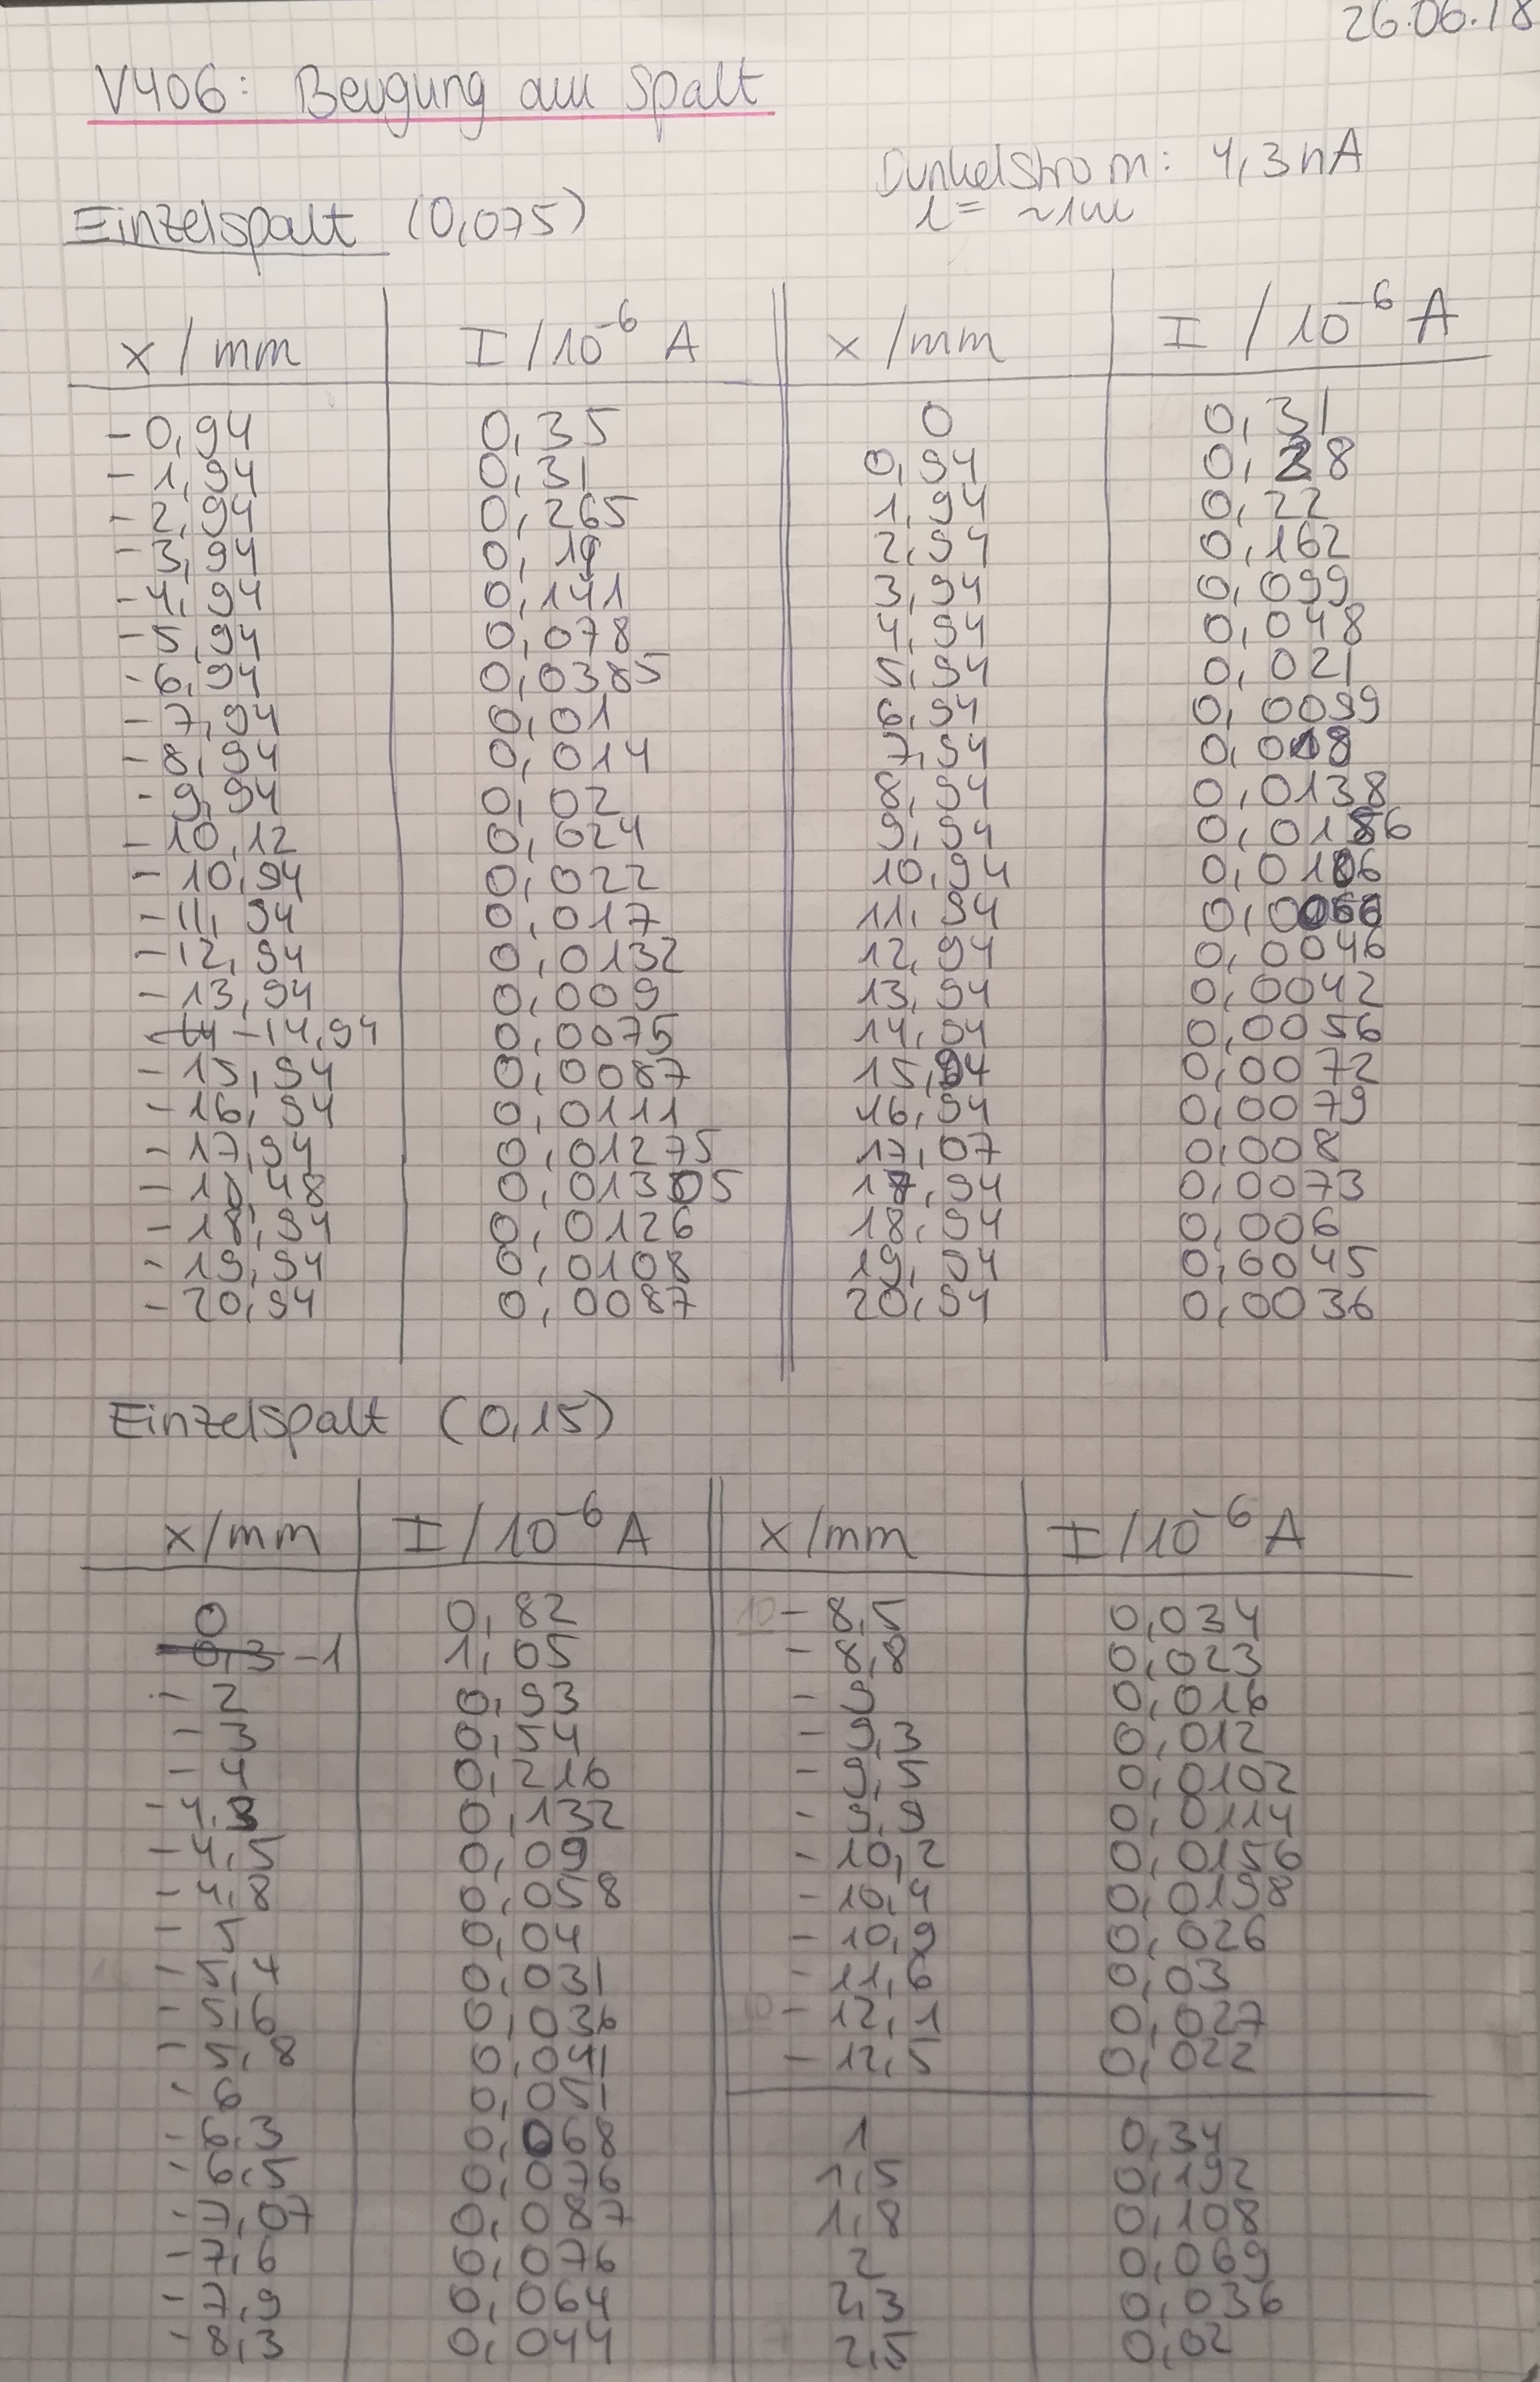
\includegraphics[width=0.9\linewidth]{../../1}
	\caption{}
	\label{fig:1}
\end{figure}
\begin{figure}[h!]
	\centering
	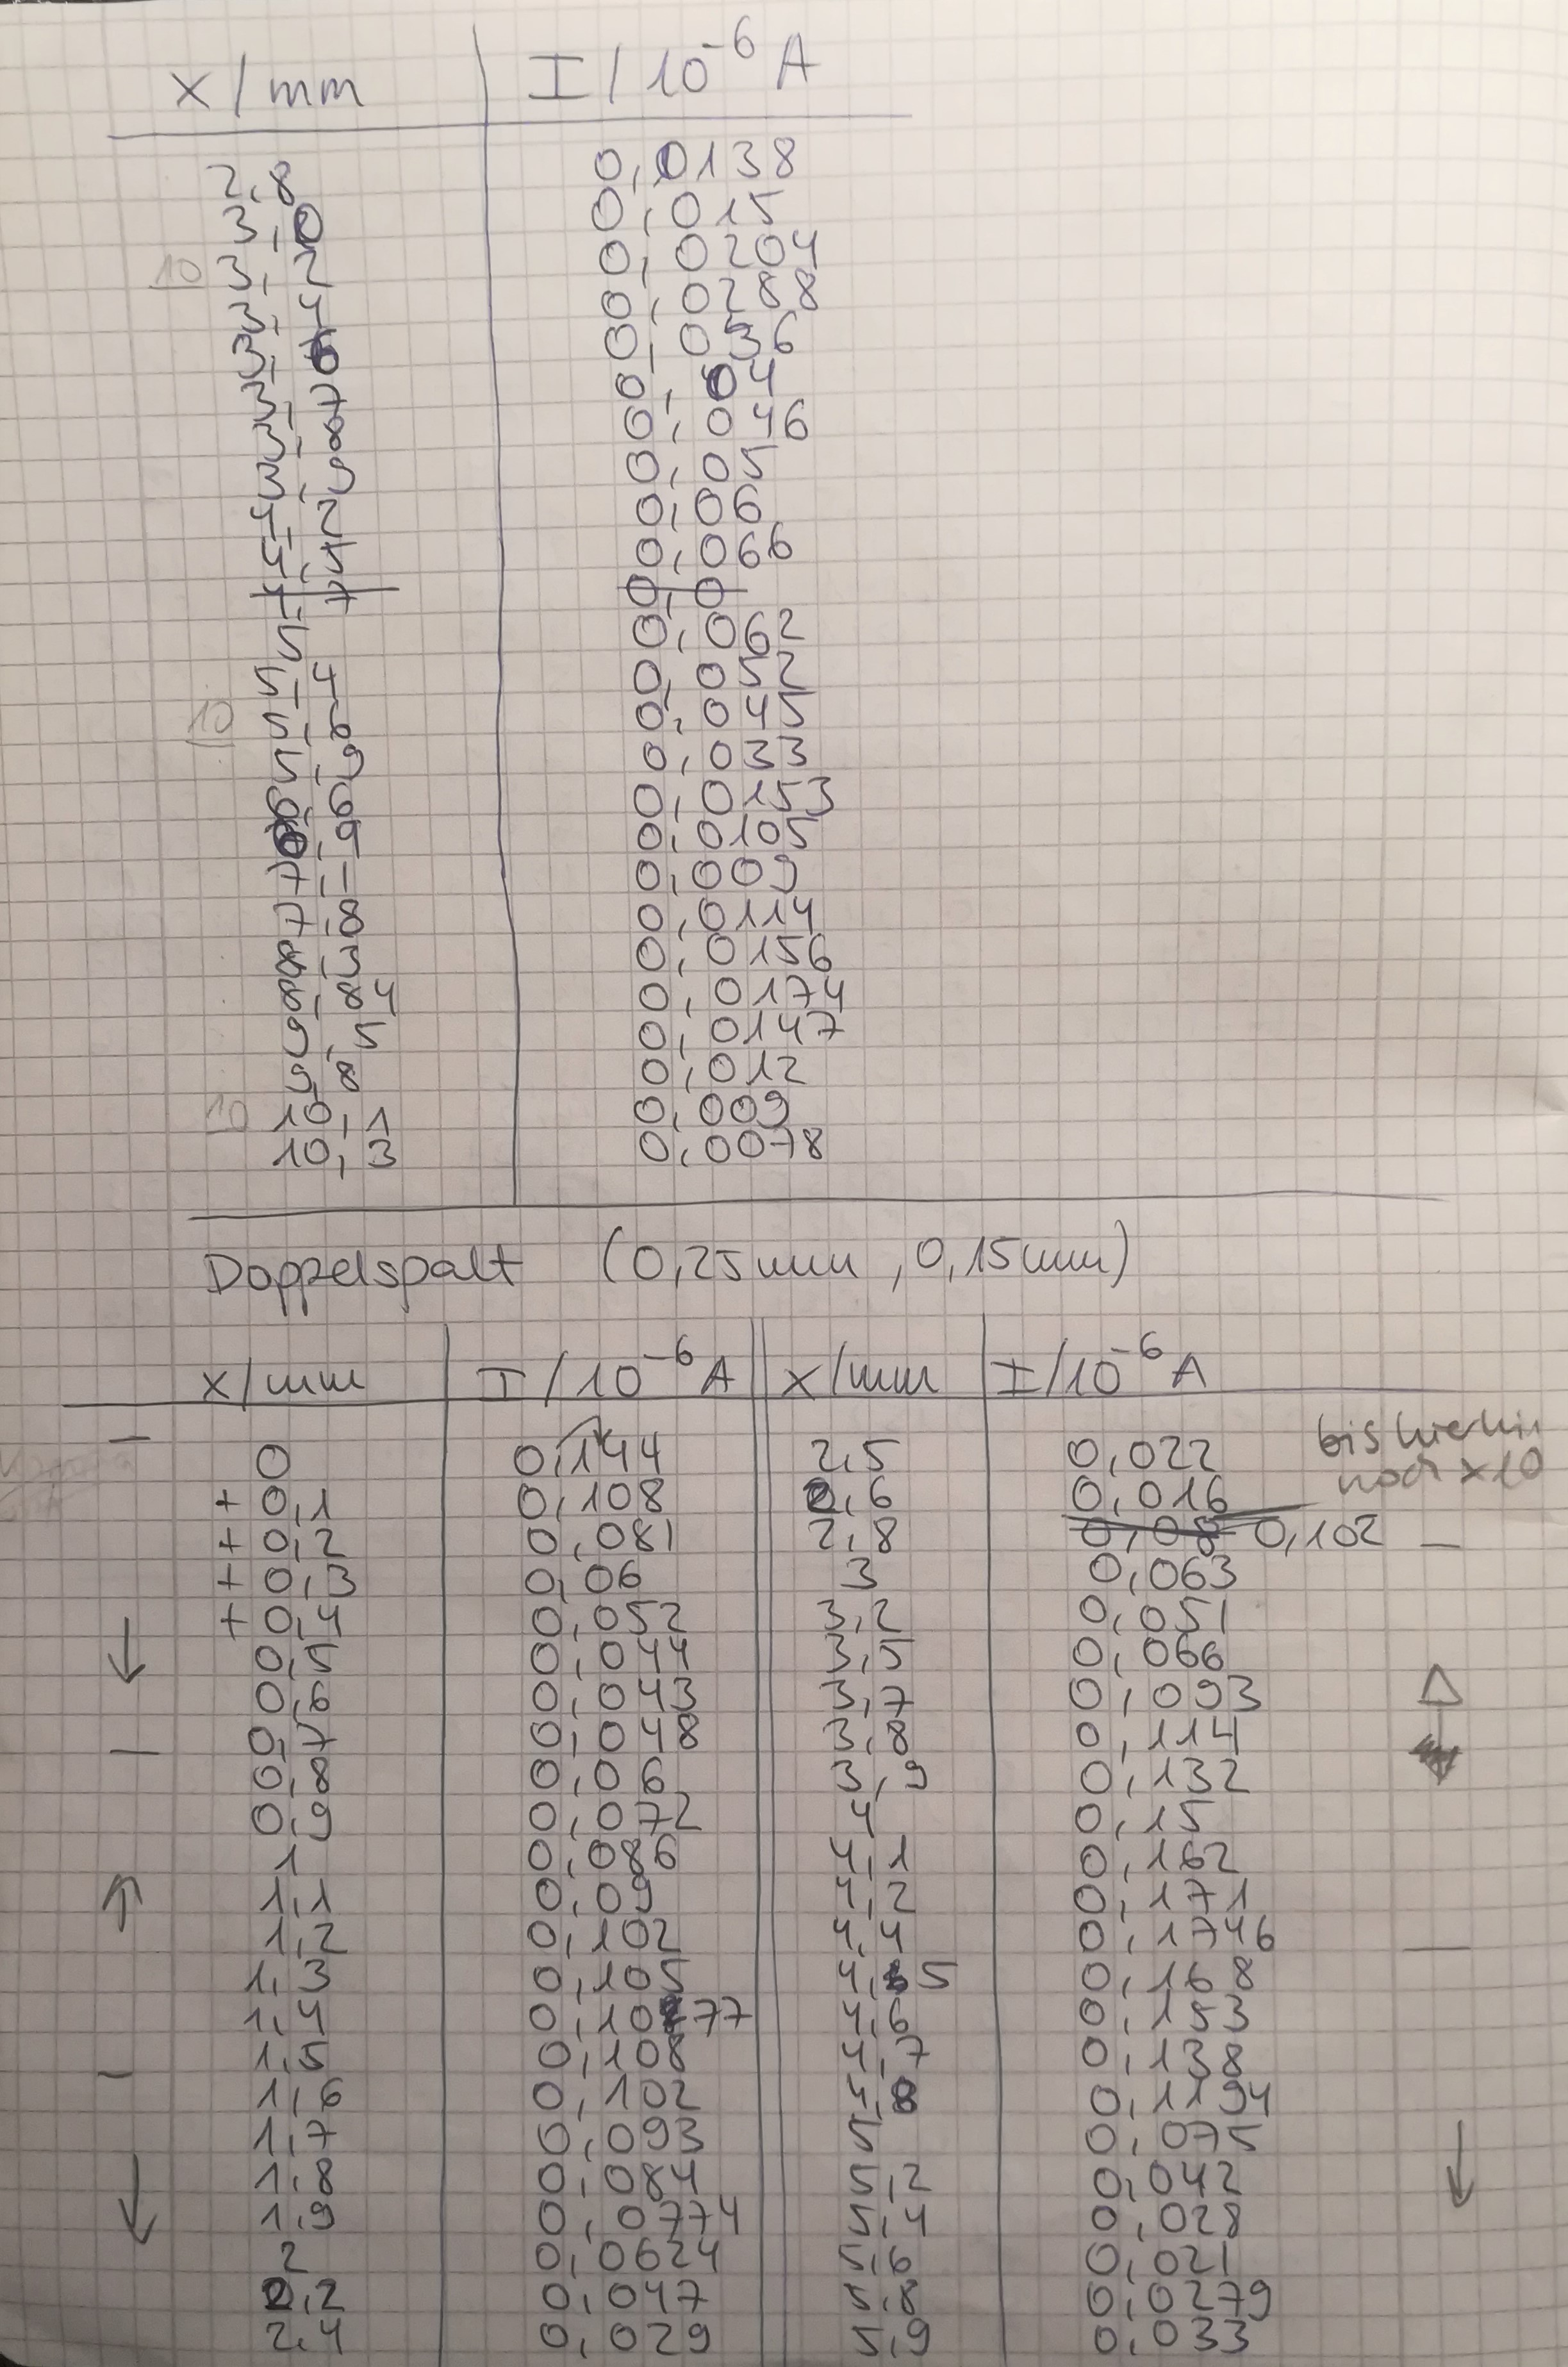
\includegraphics[width=0.9\linewidth]{../../2}
	\caption{}
	\label{fig:2}
\end{figure}
\begin{figure}[h!]
	\centering
	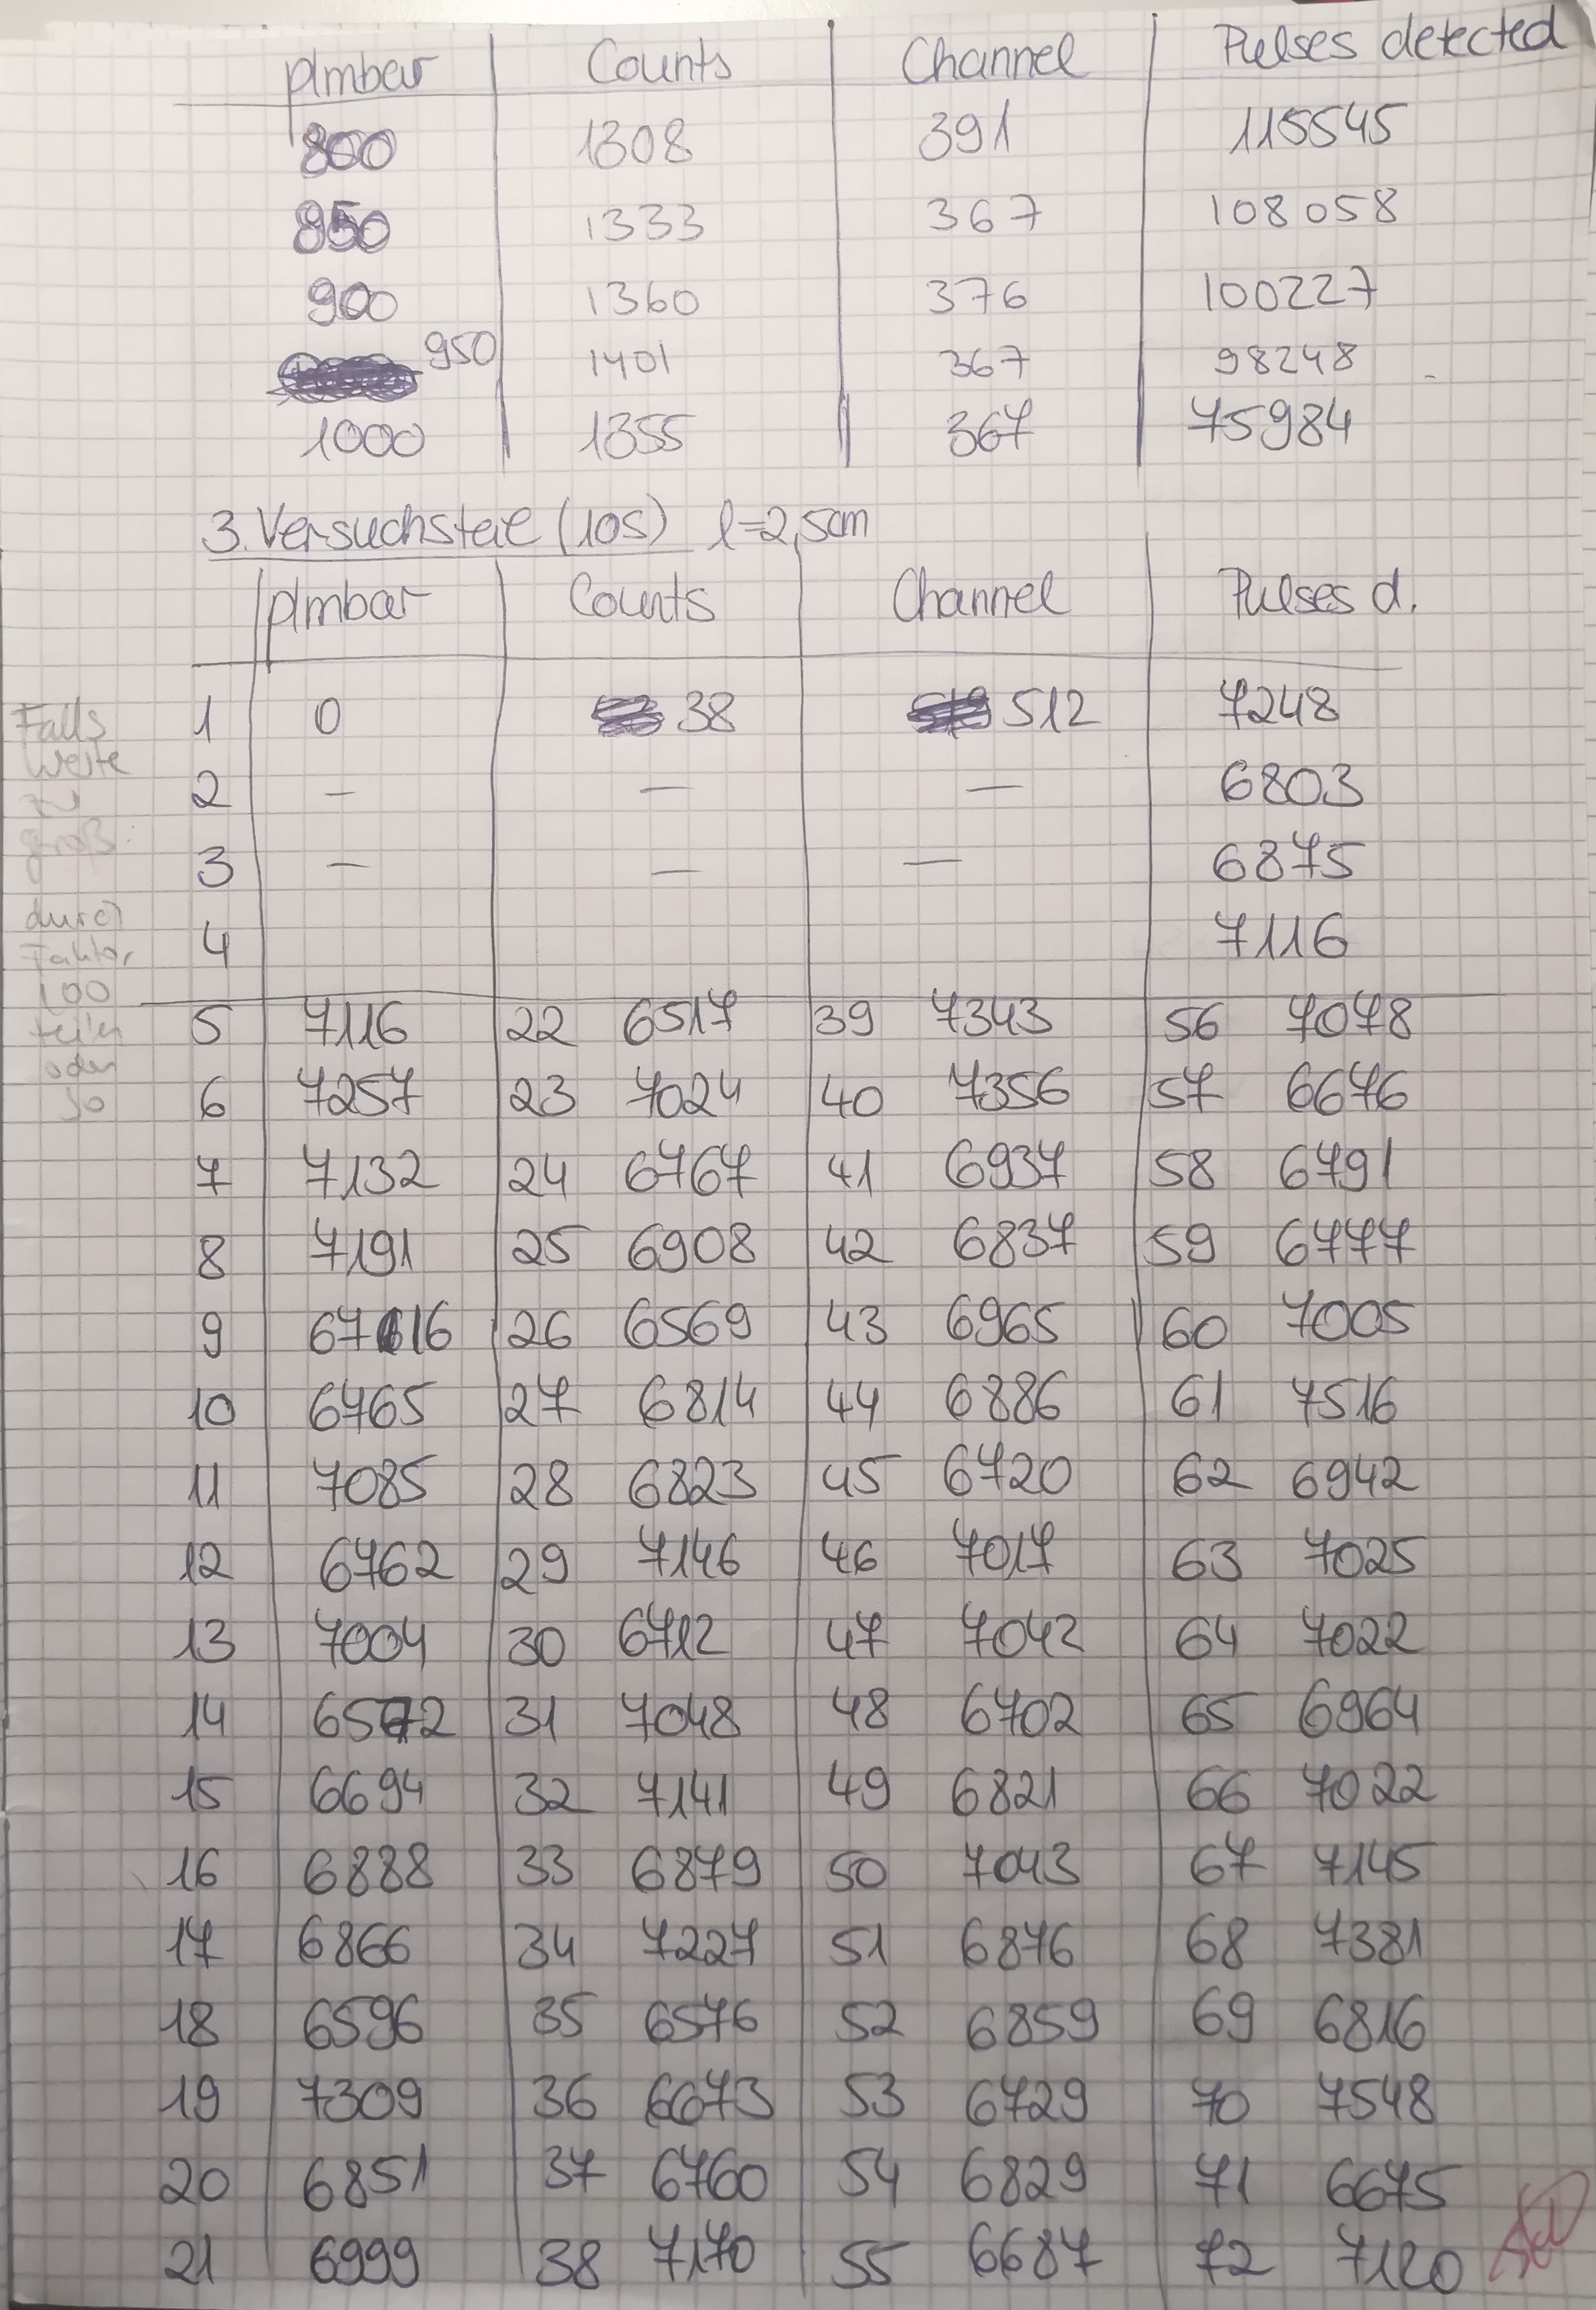
\includegraphics[width=0.9\linewidth]{../../3}
	\caption{}
	\label{fig:3}
\end{figure}
\begin{figure}[h!]
	\centering
	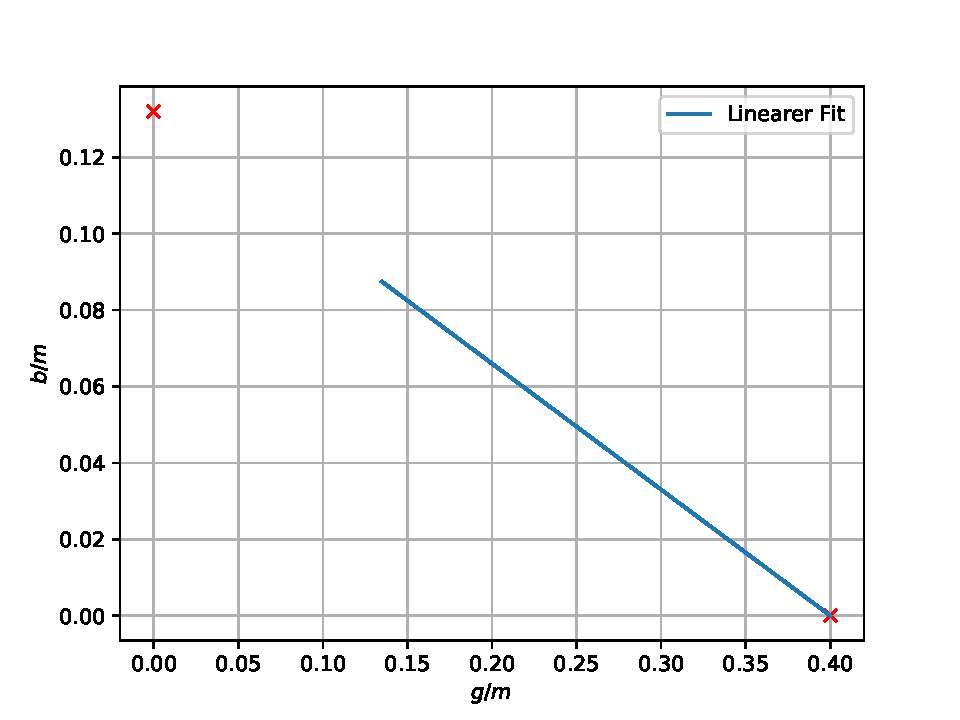
\includegraphics[width=0.9\linewidth]{../../5}
	\caption{}
	\label{fig:5}
\end{figure}
\begin{figure}[h!]
	\centering
	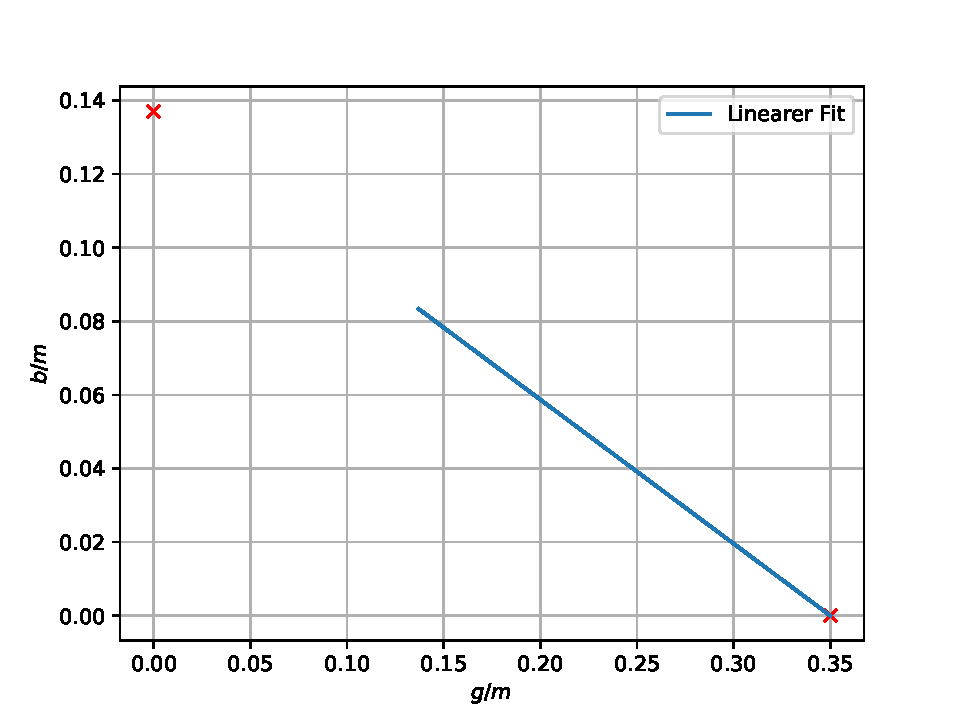
\includegraphics[width=0.9\linewidth]{../../6}
	\caption{}
	\label{fig:6}
\end{figure}
\begin{figure}[h!]
	\centering
	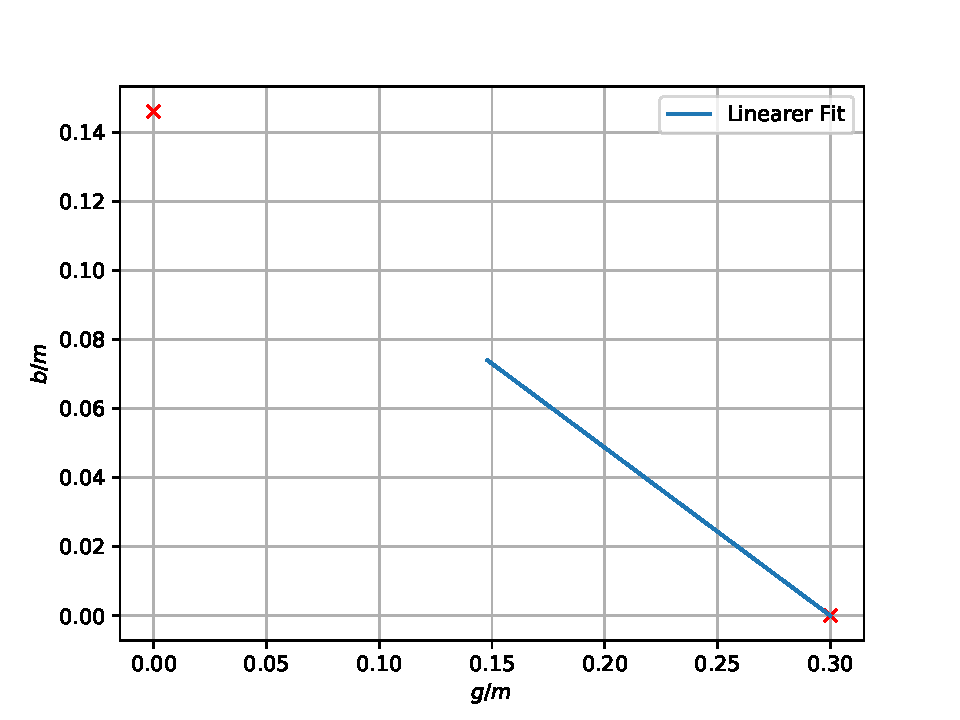
\includegraphics[width=0.9\linewidth]{../../7}
	\caption{}
	\label{fig:7}
\end{figure}
\begin{figure}[h!]
	\centering
	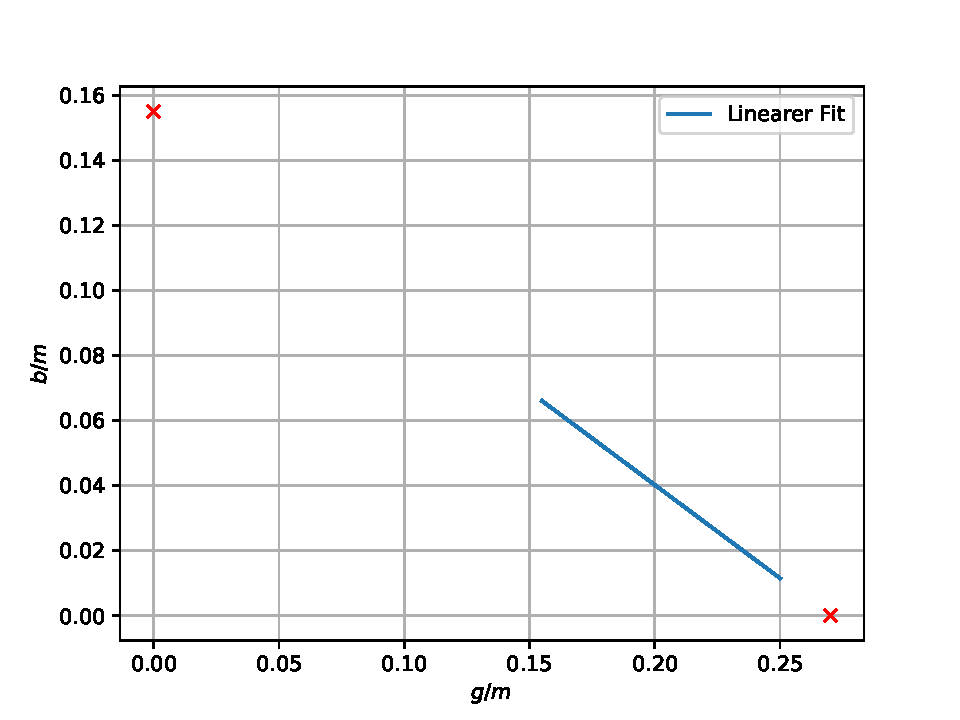
\includegraphics[width=0.9\linewidth]{../../8}
	\caption{}
	\label{fig:8}
\end{figure}

